% ---------------------------------------------------------------- Slide 40
\begin{frame}{Some perspectives\dots}
\vfill
\begin{itemize}
    \setlength{\itemsep}{1.0em}
    \item Reinforcement Learning as an Engineering Tool
    \item Reinforcement Learning and the Real World
    \item Reinforcement Learning as ``Universal'' Learning
\end{itemize}
\vfill
\end{frame}

\section{RL as an Engineering Tool}

% ---------------------------------------------------------------- Slide 41 (divider)
\begin{frame}{}
    \LARGE Reinforcement Learning as an \textbf{Engineering Tool}
\end{frame}

% ---------------------------------------------------------------- Slide 42
\begin{frame}{What we think RL is\dots}
\vfill
\begin{columns}[c]
\begin{column}{0.56\textwidth}
\centering
\begin{tikzpicture}[ic/.style={inner sep=0},
   ba/.style={-{Stealth[length=4mm]}, line width=4pt, blue!50!black}]
   \node[ic] (rb) at (0,0)   {
\includegraphics[height=2.1cm]{images/meta-rl-open/figures/icons/robot.jpg}};
   \node[ic] (ea) at (4.2,0) {
\includegraphics[height=2.1cm]{images/meta-rl-open/figures/icons/earth.jpg}};
   \draw[ba] (rb.north) to[bend left=45] (ea.north);
   \draw[ba] (ea.south) to[bend left=45] (rb.south);
   \node[align=center] at (2.1,2.45)  {decisions (actions)};
   \node[align=left, anchor=north west] at (1.0,-1.95)
        {\underline{consequences}\quad(states)\\[2pt] observations\\[2pt] rewards};
\end{tikzpicture}
\end{column}
\begin{column}{0.44\textwidth}
\centering
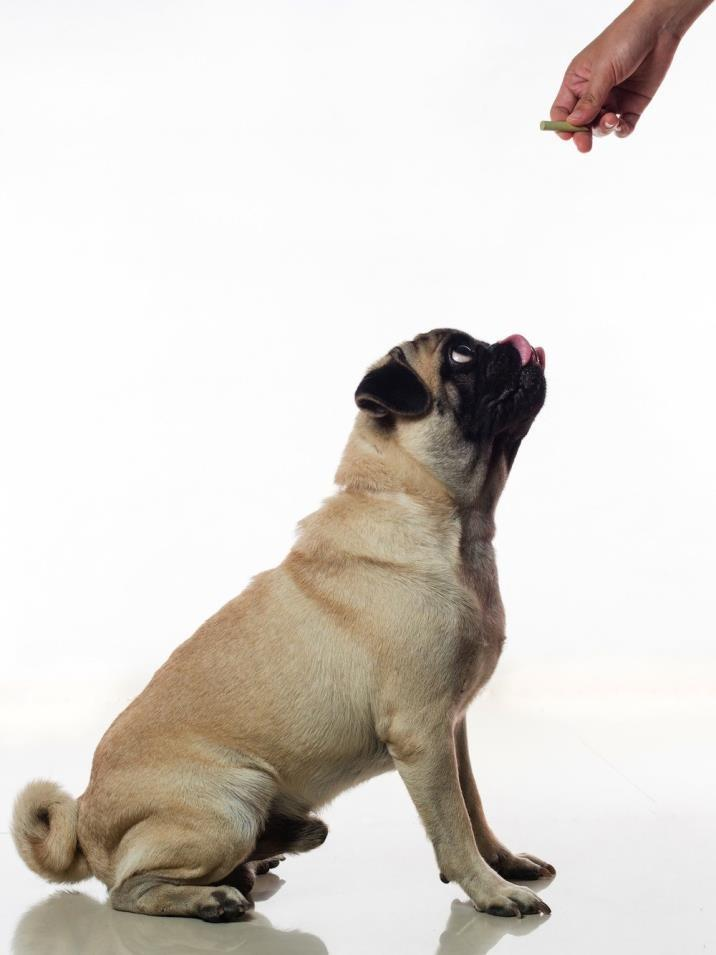
\includegraphics[height=0.72\textheight]{images/meta-rl-open/figures/dog-training.jpg}
\end{column}
\end{columns}
\vfill
\end{frame}

% ---------------------------------------------------------------- Slide 43
\begin{frame}{Engineering a control system}
\centering
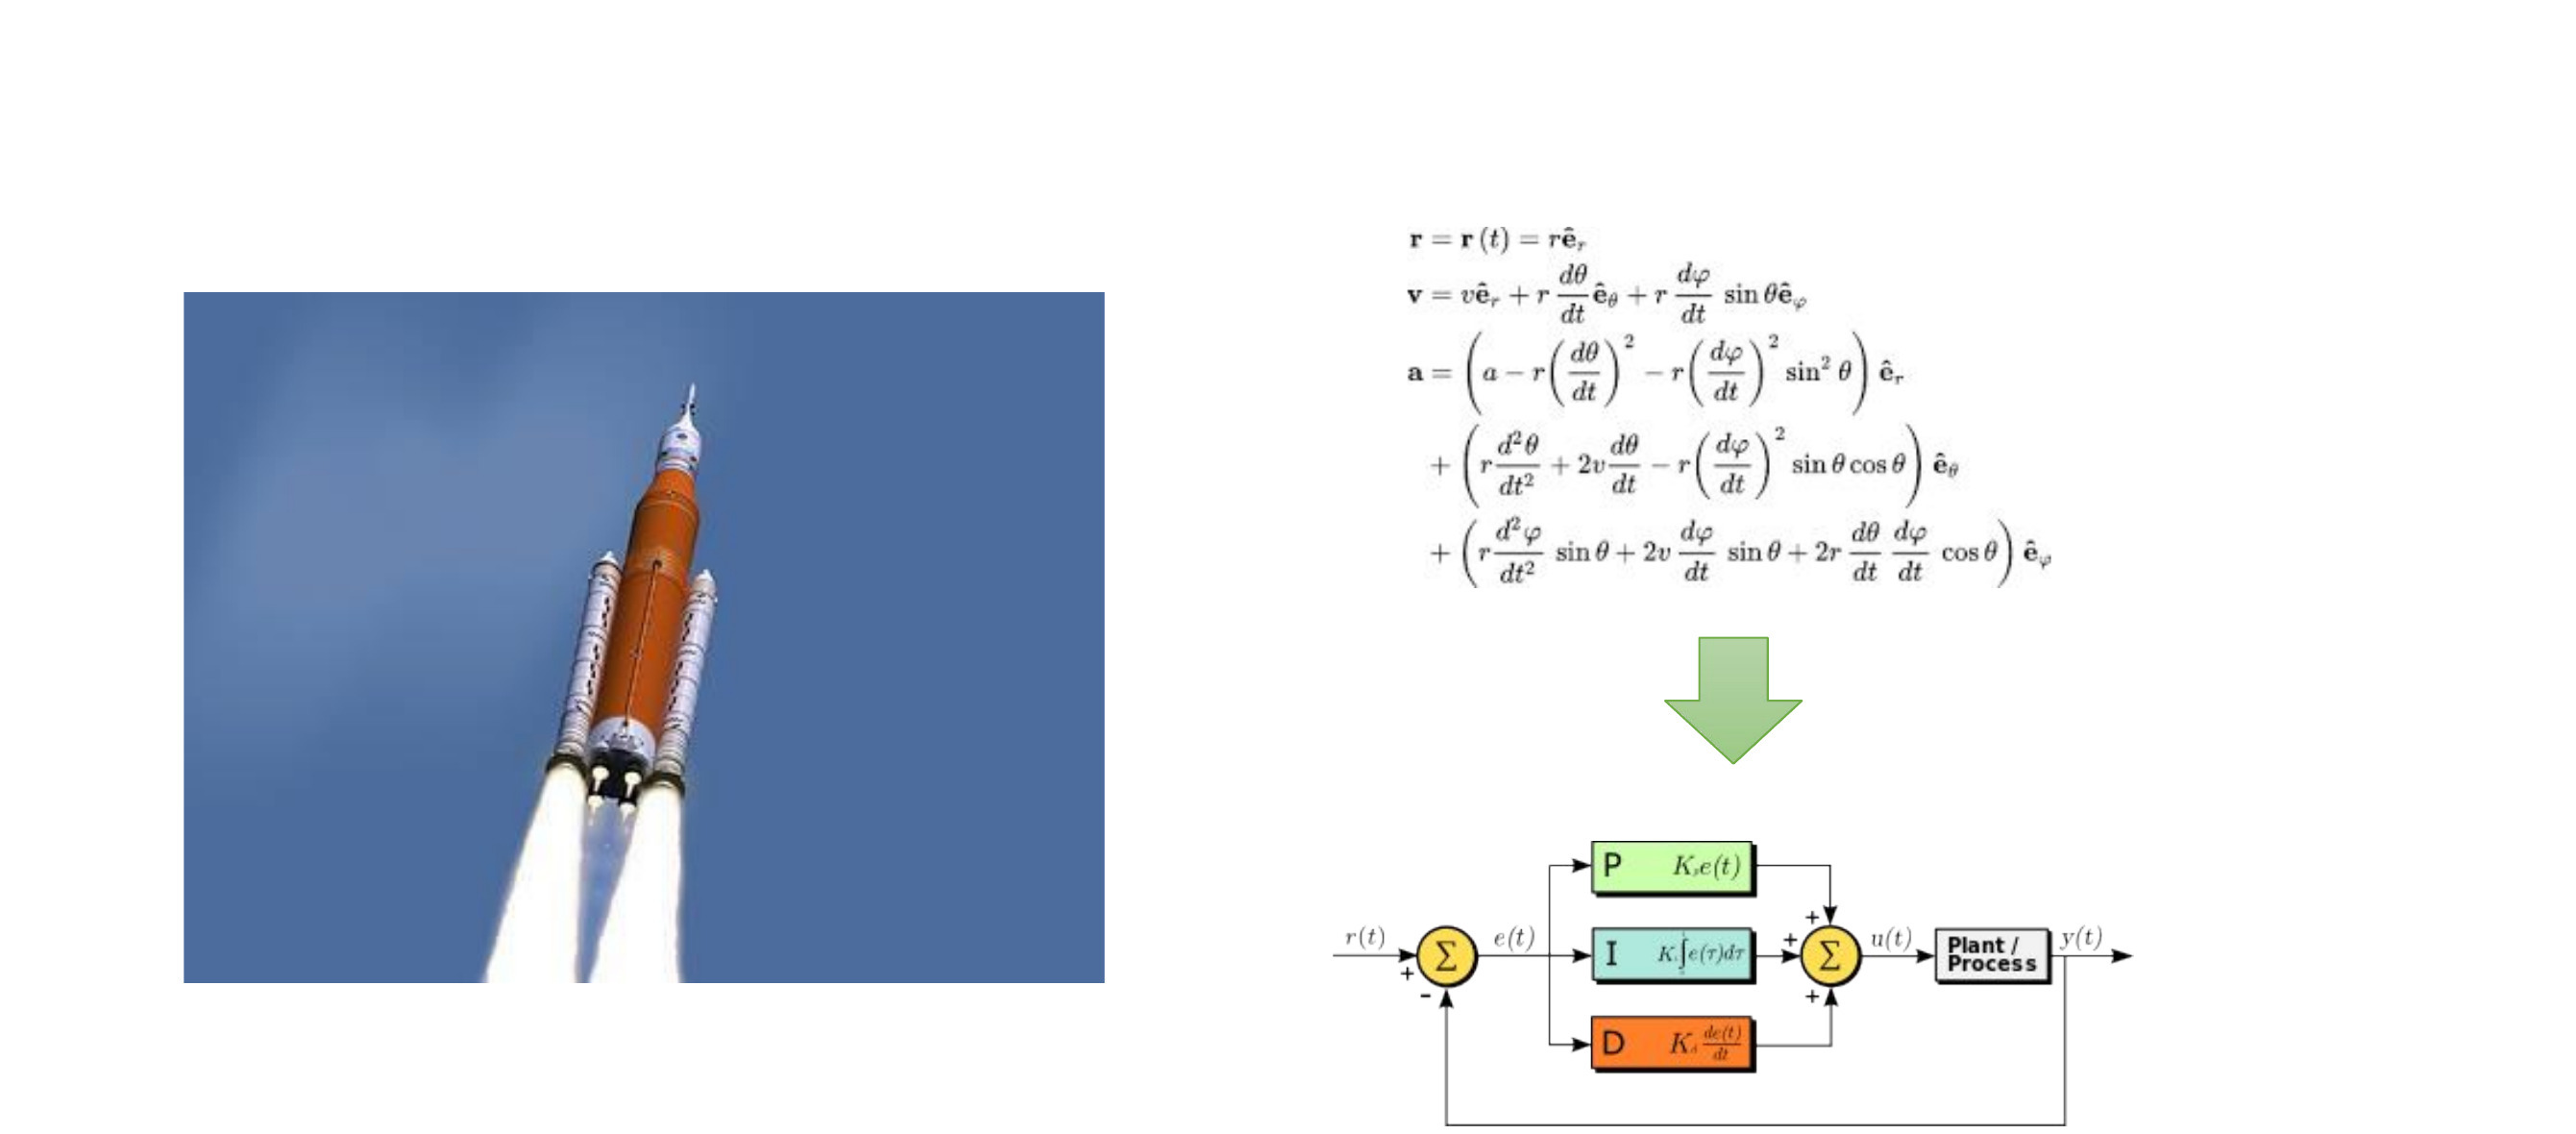
\includegraphics[width=\linewidth,height=0.82\textheight,keepaspectratio]{images/meta-rl-open/figures/control-eng.jpg}
\end{frame}

% ---------------------------------------------------------------- Slide 44
\begin{frame}{Characterization and simulation\dots}
\vfill
\begin{columns}[c]
\begin{column}{0.5\textwidth}
\centering
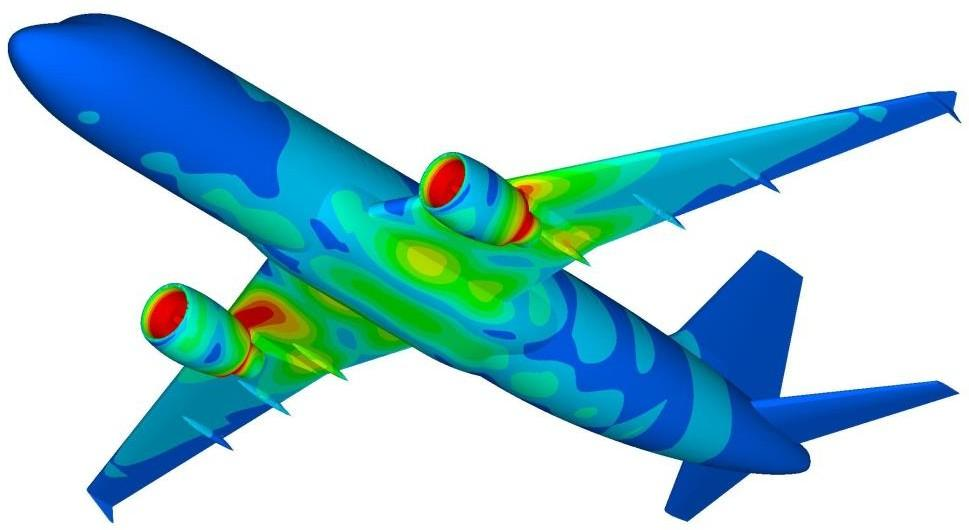
\includegraphics[width=\linewidth]{images/meta-rl-open/figures/characterization-plane.jpg}
\end{column}
\begin{column}{0.5\textwidth}
\centering
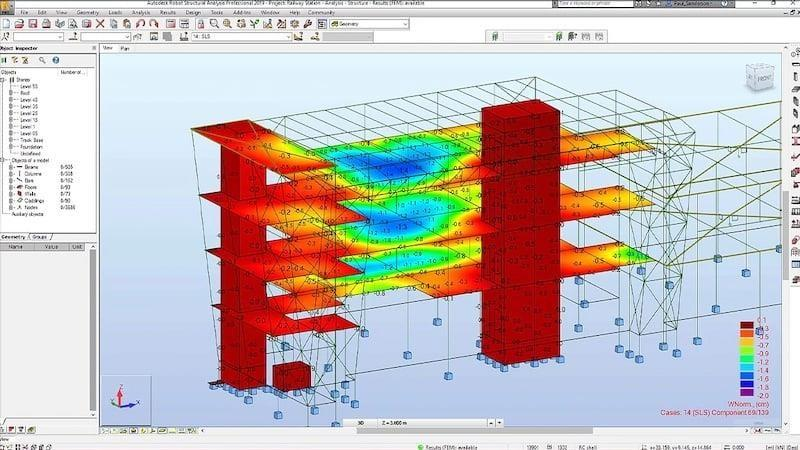
\includegraphics[width=\linewidth]{images/meta-rl-open/figures/characterization-building.jpg}
\end{column}
\end{columns}
\vfill
\end{frame}

% ---------------------------------------------------------------- Slide 45
\begin{frame}{RL: anything you can simulate you can control}
\begin{columns}[c]
\begin{column}{0.6\textwidth}
\begin{itemize}
    \item Provides a powerful engineering tool
    \item Not that different from conventional engineering approach!
    \begin{itemize}
        \item Before: characterize, simulate, control
        \item Now: characterize, simulate, run RL
    \end{itemize}
    \item Main role: powerful inversion engine
    \item Main weakness: still need to simulate!
\end{itemize}
\end{column}
\begin{column}{0.4\textwidth}
\centering
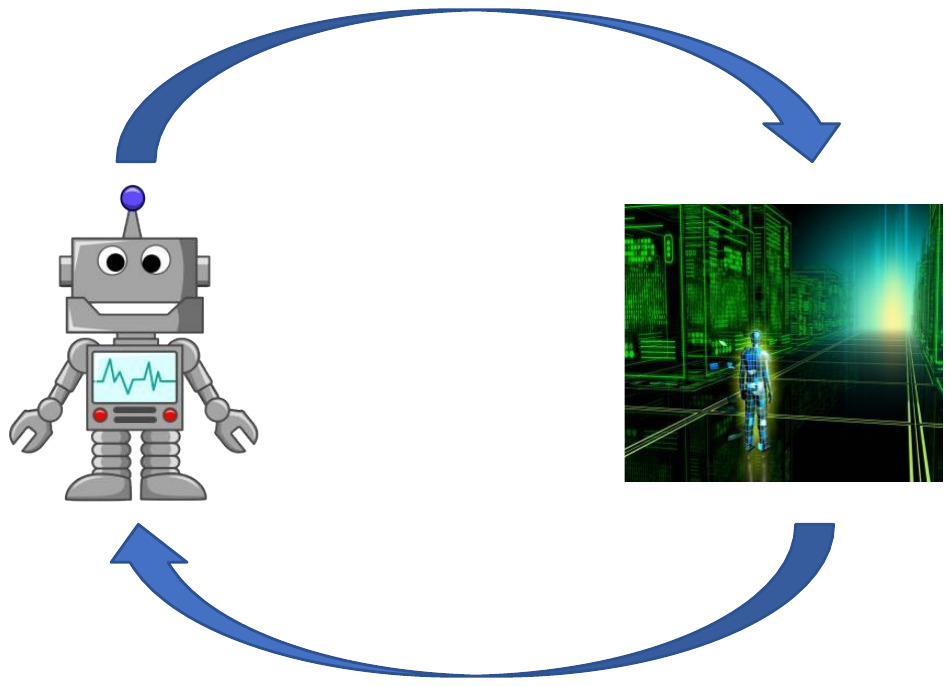
\includegraphics[width=\linewidth]{images/meta-rl-open/figures/simulate-control.jpg}
\end{column}
\end{columns}
\end{frame}
